%%%%%%%%%%%%
%% Please rename this main.tex file and the output PDF to
%% [lastname_firstname_graduationyear]
%% before submission.
%%%%%%%%%%%%

\documentclass[12pt]{caltech_thesis_finalreport}
\usepackage[hyphens]{url}
\usepackage{lipsum}
\usepackage{graphicx}
%\usepackage{svg}
\usepackage{todonotes}

\usepackage{dirtytalk}
\graphicspath{{images/}}
\usepackage{float}
\usepackage{hyperref}
\hypersetup{
    colorlinks,
    linkcolor={red!50!black},
    citecolor={blue!50!black},
    urlcolor={blue!80!black}
}
\renewcommand{\chaptername}{}
\AtBeginDocument{\renewcommand{\bibname}{References}}
%% Tentative: newtx for better-looking Times
\usepackage[utf8]{inputenc}
\usepackage[T1]{fontenc}
%\usepackage{newtxtext,newtxmath}
%\usepackage{newtxmath}
\usepackage{amsmath}
\usepackage{amsfonts}
\usepackage[backend=bibtex,
style=numeric,
bibencoding=ascii,
sorting=none
%style=alphabetic
%style=reading
]{biblatex}

%\renewcommand{\familydefault}{\rmdefault}
% Must use biblatex to produce the Published Contents and Contributions, per-chapter bibliography (if desired), etc.
% Name of your .bib file(s)
\addbibresource{example.bib}
\addbibresource{ownpubs.bib}

\begin{document}

% Do remember to remove the square bracket!
\title{Information-Performance Tradeoffs in Control}
\author{Ayush Pandey}

%\degreeaward{Visiting Undergraduate Research Program}                 % Degree to be awarded
\university{California Institute of Technology}    % Institution name
\address{Pasadena, California}  
	                   % Institution address
\unilogo{caltech.png}                                 % Institution logo
\copyyear{Oct 2016}  % Year (of graduation) on diploma
\defenddate{17th Oct}          % Date of defense
%
%\orcid{[Author ORCID]}

%% IMPORTANT: Select ONE of the rights statement below.
%\rightsstatement{All rights reserved\todo[size=\footnotesize]{Choose one from the choices in the source code!! And delete this \texttt{todo} when you're done that. :-)}}
% \rightsstatement{All rights reserved except where otherwise noted}
% \rightsstatement{Some rights reserved. This thesis is distributed under a [name license, e.g., ``Creative Commons Attribution-NonCommercial-ShareAlike License'']}

%%  If you'd like to remove the Caltech logo from your title page, simply remove the "[logo]" text from the maketitle command
\maketitle[logo]
%\maketitle

%\begin{acknowledgements} 	 
%   [Add acknowledgements here. If you do not wish to add any to your thesis, you may simply add a blank titled Acknowledgements page.]
%\end{acknowledgements}
%
%\begin{abstract}
%   [This abstract must provide a succinct and informative condensation of your work. Candidates are welcome to prepare a lengthier abstract for inclusion in the dissertation, and provide a shorter one in the CaltechTHESIS record.]
%\end{abstract}

%% Uncomment the `iknowhattodo' option to dismiss the instruction in the PDF.
%\begin{publishedcontent}%[iknowwhattodo]
%% List your publications and contributions here.
%\nocite{Cahn:etal:2015}
%\end{publishedcontent}

\tableofcontents
%\listoffigures
%\listoftables
%\printnomenclature

\mainmatter

\chapter{Introduction}
\label{intro}
	Over the past few decades the fields of communication and control have been developed extensively to support the emerging needs of the society such as higher speed internet, better telephone communication networks, wireless access to devices over Internet of Things (IoT), reliable long distance satellite communication, home automation and many other related fields. While communication theory is mainly concerned with the transmission of information from one point to another reliably it does not deal with what is done with the information once it is transmitted. Control theory, on the other hand, mainly deals with using the information it receives as feedback in order to achieve better performing systems, which are not prone to disturbances, noises and other process variations. Although there is substantial research on control and information theory, the research on networked control systems (control systems with communication between its components) is still in a nascent stage.\\
Networked control systems are increasingly finding wide applications but they also pose newer challenges which are neither addressed in control theory nor in information theory. The components of a networked control system are physically distributed with communication links between the plant, controller, observer and/or the actuators. These links connecting the different components are often noisy and pose various other constraints (See \cite{constraints} for details). Hence, the control design and analysis needs to be done keeping in mind these information bottlenecks. In control system design, it is usually desired to minimize a performance index. Because of the information bottlenecks, there exists a tradeoff between the best achievable performance and the observation accuracy (it is intuitive that worse the observation accuracy, worse would be the performance of the system). 
We dealt with two important settings of networked control systems in this project:
\begin{enumerate}
\item Noiseless rate-limited communication of data between observer and controller 
\item Communication over Additive White Gaussian Noise (AWGN) channel between the observer and the controller.
\end{enumerate} 
\chapter{Background}
Throughout this paper, unless otherwise mentioned, we deal with a Linear Quadratic Gaussian (LQG) control system setting with a communication link between the observer and the controller. This section covers LQG control theory very briefly and introduces the two communication constraints --- rate-limited channel and AWGN channel in the feedback path.

	\subsection{Classical Partially Observed LQG Problem}
	For a stochastic system, the LQG control scheme estimates the states from the available outputs. Using this estimation of states a controller is designed such that a quadratic performance index is minimized. Consider a discrete time stochastic system, the state equation can be written as
	\begin{align}
	\label{systemeq}
	x_{t+1} &= A_{t}x_{t}+ B_{t}u_{t} + w_{t}\\
	\intertext{The output equation is}
	y_{t}&=C_{t}x_{t}+v_{t}
	\end{align}
	where $w_{t}$ and $v_{t}$ are assumed to be zero mean Gaussian noises with covariances $W_{t}$ and $V_{t}$ in process and measurement respectively. For states $x_{t} \in \mathbb{R}^{n \times 1}$, inputs $u_{t} \in \mathbb{R}^{k \times 1}$ and outputs $y_{t} \in \mathbb{R}^{p \times 1}$ we have, the stochastic state transition matrix $A_{t} \in \mathbb{R}^{n \times n}$, the stochastic control multipliers, $B_{t} \in \mathbb{R}^{n \times k}$ and the stochastic output multipliers, $C_{t} \in \mathbb{R}^{p \times n}$. We also assume that the distribution of the initial value of the state $x$, $x_{0}$ is known and that $w,v$ and $x_{0}$ are all independent of each other. The system is stationary which ensures that the mean and covariances will not change with time. The following block diagram representation gives a clearer picture of LQG control.
	\begin{figure}[H]

			  \centering
%			  \includesvg[width=1.0\textwidth]{block2}
%			  \def\svgscale{5.5}
			  \tiny{
			  \resizebox{10cm}{!}{\input{lqg_block.pdf_tex}}}
%			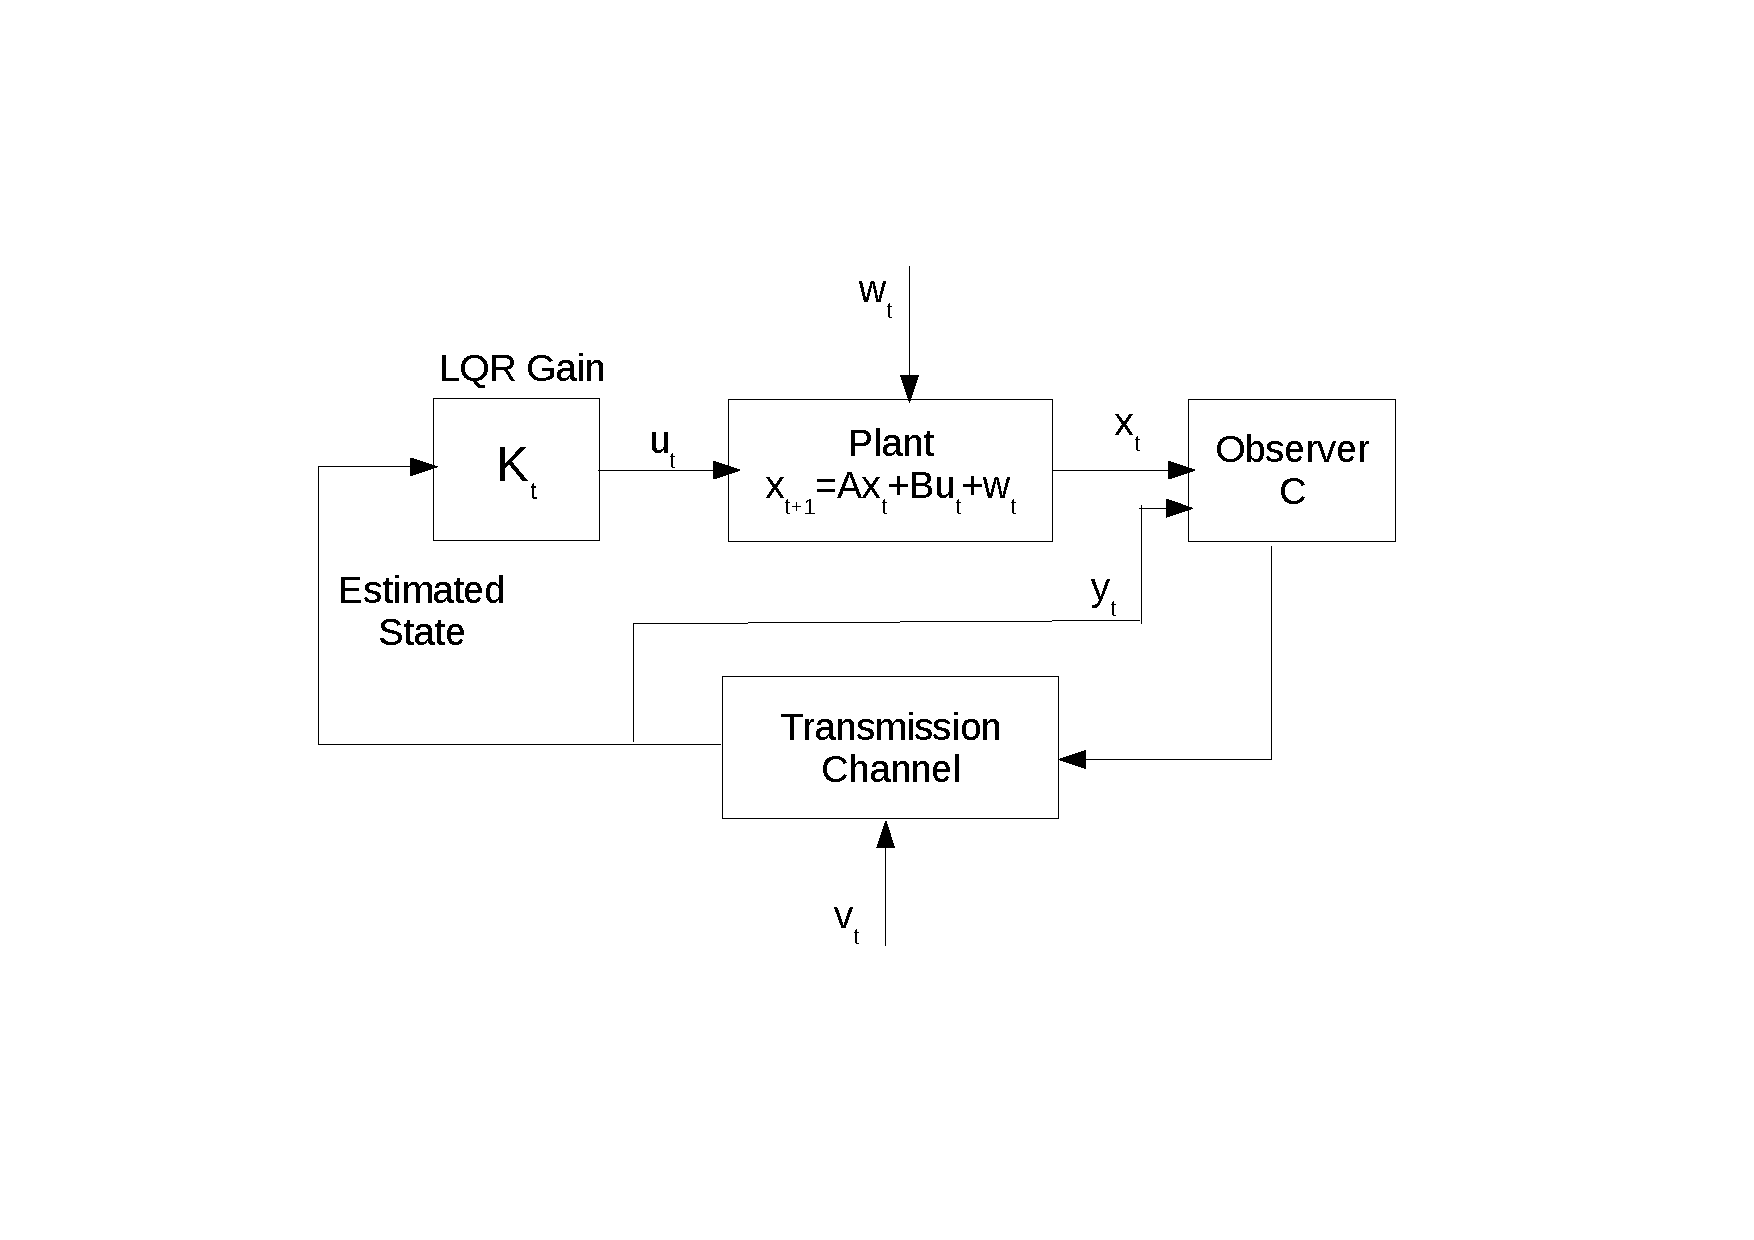
\includegraphics[scale=0.5]{lqg_block}
%			\includesvg[width=10cm]{lqg_block}
			  \caption{Representative Block Diagram of Classical Partially Observed LQG Control}
			 \label{lqg}
		\end{figure}	
	
	The aim is to find a control law $u_{t}$ so that the following performance index is minimized, where $Q \geq 0$ is the state weighting matrix and $R > 0$ is the control weight matrix. 
	\begin{align}
		b(\cdot)&=E\left(\sum\limits_{t=0}^{N-1} \left(x_{t}^{T}Qx_{t} + u_{t}^{T}Ru_{t}\right) + x_{N}^{T}Qx_{N} \right)\\
	\intertext{The control law is given by}
	\label{controleq}
	u_{t}&=-L_{t}E[x_{t}|y_{1},y_{2},...,y_{t}]
	\end{align}
	 where $L_{t}$ is the LQR gain and $E[x_{t}|y_{1},y_{2},...,y_{t}]$ is the minimum mean square error estimate of $x_{t}$ given that all past output measurements are available. It can be proved that the calculation of the LQR gain $L_{t}$ and the MMSE estimate of the state using Kalman Filter can be performed independent of each other \cite{book}. 
	\subsection{Rate-Limited Communication Channel}
	If in Fig.(\ref{lqg}) the observer data is transmitted via a digital communication link to the controller then the system performance would also be dependent on the data rate at which this communication is done. Hence, there exists a tradeoff between communication rate and optimal performance (faster the rate, better the performance). \\We studied the tightness of the bounds on the performance cost for the rate-limited noiseless communication channel using different quantization schemes. The information-theoretic lower and upper bounds have been given in \cite{victoria}. We also considered a system where the system matrix $A$ (see Eq.(\ref{systemeq})) is uncertain but has a known probability distribution. 
	\subsection{Additive White Gaussian Channel}
We studied a system where the observations are corrupted by additive white Gaussian noise during the transmission from the observer to the controller, which is often the case when analog communication is used to transmit information.
Continuing on the work in the recent paper \cite{anatoly} where the system disturbances $w$ (See Eq.(\ref{systemeq} )) have been assumed to have Gaussian distribution, we instead dealt with other probability distributions of $w$. We tried to show that the information-theoretic bounds (as given in \cite{victoria}) are tight even when $w$ is not Gaussian.
\chapter{AWGN Communication Constraint}
Consider the scalar system in Eq.(\ref{systemeq}) but with communication over AWGN channel between observer and the controller. Using controller and estimator (Kalman Filter) Algebraic Riccati Equations (AREs) (see \cite{anatoly} and \cite{lqg}) we have the expressions for the controller gain $L(t)$ and Kalman gain $P(t)$ for the control over AWGN channel case.
\begin{align}
P(t+1) &= A^{2}P(t)\left(1 - \left(\frac{P(t)}{P(t) + 1}\right)\left(\frac{SNR}{SNR + 1}\right)\right) + W\\
S(t) &= \frac{A^{2}RS(t+1)}{S(t+1) + R} + Q\\
L(t) &= \frac{AS(t+1)}{S(t+1) + R}\\
\intertext{Using the above, the expression for optimal cost($b^{*}$) achieved vs SNR of the channel was derived as follows.}
	\label{computedJ}
	 b^{*}(\cdot) &= \sum\limits_{t = 0}^{T} \left[Q\Sigma(t) + \left(S(t)\left(A^{2}\Sigma(t-1) + W - \Sigma(t)\right)\right)\right]\\
	 \intertext{where $\Sigma(t)$ can be obtained using Kalman filter gains $P(t)$ as follows}
	 \Sigma(t) &= \frac{P(t)-W}{A^{2}}
	\end{align}
%The resulting plot for a fully observable system ($v = 0$) is shown in Fig.(\ref{comp_vs_sim}). 
%		\begin{figure}[H]
%			 \centering
%%			
%				\tiny{
%%			  \resizebox{5in}{!}{\input{lowerBound_Simulation_rateLimitedLQG.pdf_tex}}
%			\includesvg[width=16cm]{computed_vs_simulated_snr30_manyTime}}
%%			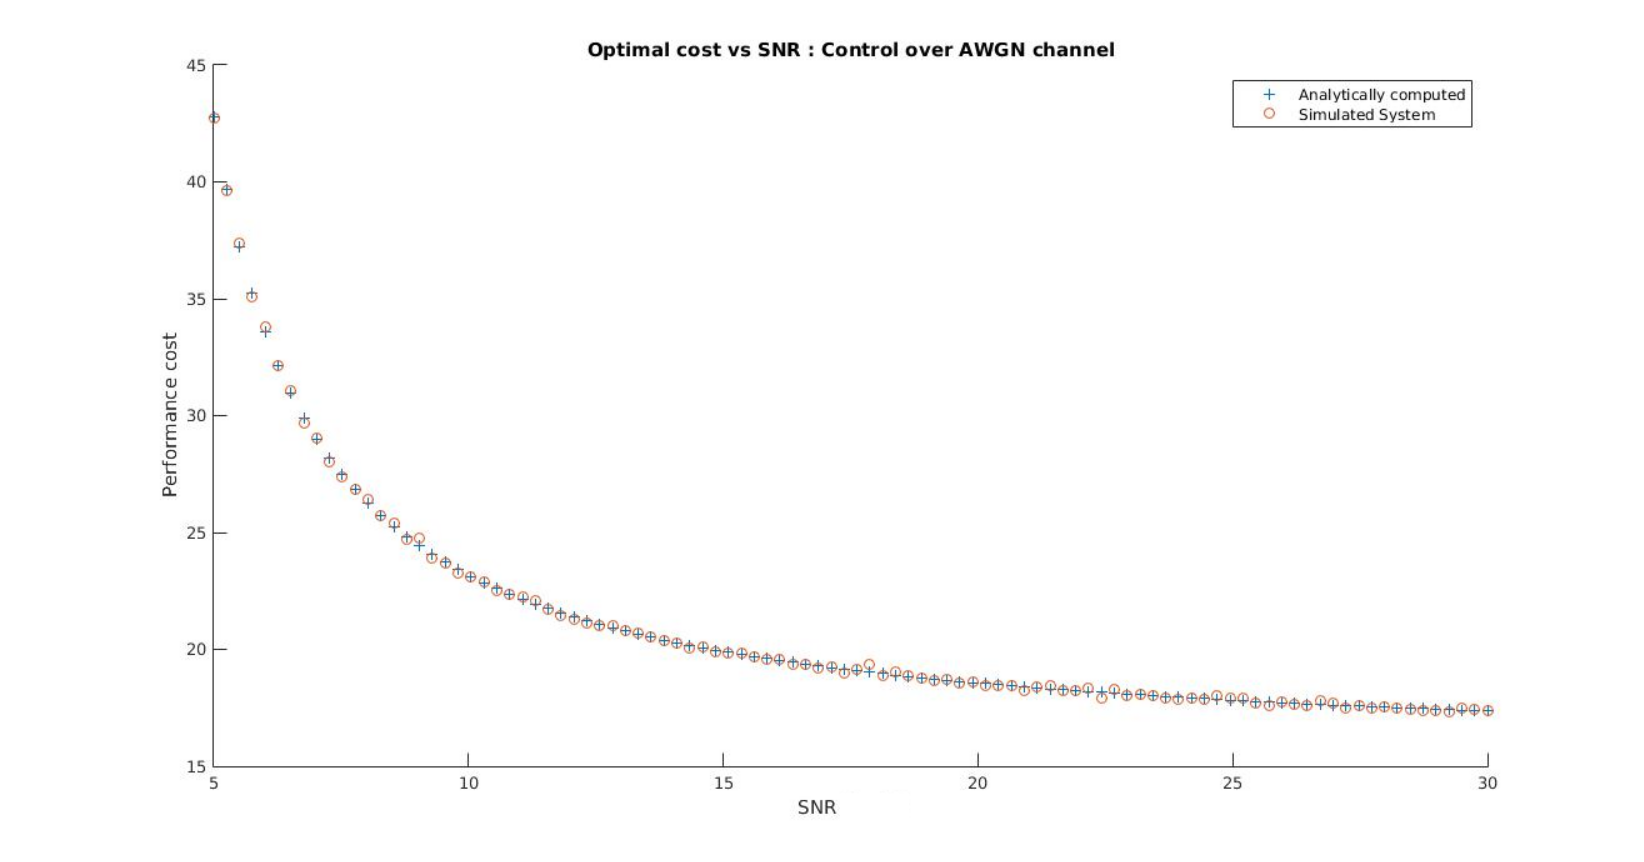
\includegraphics[scale=0.27]{computed_vs_simulated_snr30_manyTime}
%					  
%			  \caption{Comparing the computed optimal cost with the simulated optimal cost for system with AWGN communication channel. The fully observable system has the parameter $A = 2$ and the system disturbance $w$ is zero mean Gaussian with $\sigma_{w} = 1$.}			 
%			 \label{comp_vs_sim}
%		\end{figure}	
%Similarly, for partially observable case with Gaussian noise $v$ in measurement (i.e. $y = x + v$), we make the appropriate changes and compare the computed and the simulated optimal performance cost vs SNR on the same plot. The resulting plot is shown in Fig.(\ref{comp_vs_sim_v}).
%	\begin{figure}[H]
%			  \centering
%			\tiny{	
%%			  \resizebox{5in}{!}{\input{lowerBound_Simulation_rateLimitedLQG.pdf_tex}}
%			\includesvg[width=16cm]{control_over_AWGN_withV_GaussianW}}
%%			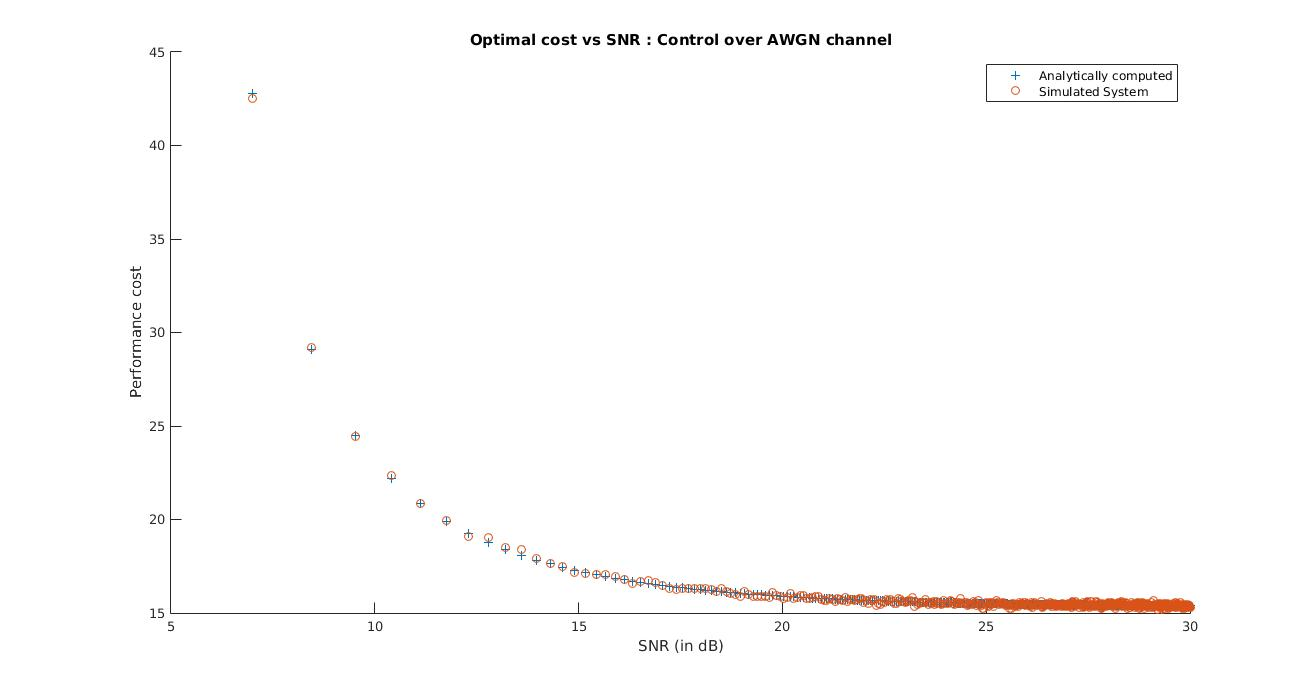
\includegraphics[scale=0.27]{computed_vs_simulated_SNRdB30}
%			  \caption{Comparing the computed optimal cost with the simulated optimal cost for system with AWGN communication channel. The partially observable system has the parameter $A = 2$, the system disturbance $w$ is zero mean Gaussian with $\sigma_{w} = 1$ and the noise in measurement $v$ is also zero mean Gaussian with $\sigma_{v} = 1$.}
%			 \label{comp_vs_sim_v}
%		\end{figure}	
		To tackle the problem of non-Gaussian system disturbance $w$, we used the result derived in \cite{victoria}. The following equation taken from \cite{victoria} gives the lower bound to the rate distortion function in terms of optimal cost $b$. 
	\begin{align}
	\label{lowerbound}
	\mathbb{R}(b) &\geq \log(|det(A)|) + \frac{n}{2} \log \left( 1 + \frac{N(w)|det(M)|^{\frac{1}{n}}}{(b-b_{min})/n}\right) \\	
	\intertext{where $b_{min}$ is the minimum cost as calculated for the classical LQG case (without communication), $N(w)$ is the entropy power given by}	
	N(w) &= \frac{1}{2 \pi e} exp \left( \frac{2}{n} h(w) \right)\\	
	\intertext{where $h(w)$ is the differential entropy of $w$ and $M$ can be obtained by solving the following Algebraic Riccati Equation (ARE):}
	S &= Q + A^{T}(S - M)A\\
	M &= SB(R + B^{T}SB)^{-1}B^{T}S\\
	\intertext{For the scalar case with $n = 1$, we have}
	\mathbb{R}(b) &\geq \log|A| + \frac{1}{2} \log \left( 1 + \frac{N(w)|M|}{b-b_{min}}\right)
	\end{align}\\		
	Using Shannon's channel capacity we used the above bound for the AWGN channel case that we are concerned with here. The lower bound given in Eq.(\ref{lowerbound}) is valid for any distribution of system disturbance $w$. The channel capacity for noise corrupted channel is given by
	\begin{equation}
		\mathbb{C} = \frac{n}{2} \log\left( 1 + SNR \right)
	\end{equation}
	where SNR is the signal to noise ratio of the AWGN channel.
	 \\To study the tightness of the lower bound given in Eq.(\ref{lowerbound}) we simulated the system and compared it with the lower bound plot. The result is shown in Fig.(\ref{lowerbound_vs_laplace}). We used a Laplace distribution for $w$ (with zero mean and $\sigma_{w} = 1$) to simulate the system and to calculate the lower bound. 
		\begin{figure}[H]
			  \centering
%			 \tiny{	
			  \resizebox{15cm}{!}{\input{laplaceW_bound_simulation_withoutV.pdf_tex}}
%			\includesvg[width=20cm]{laplaceW_bound_simulation_withoutV}}
%			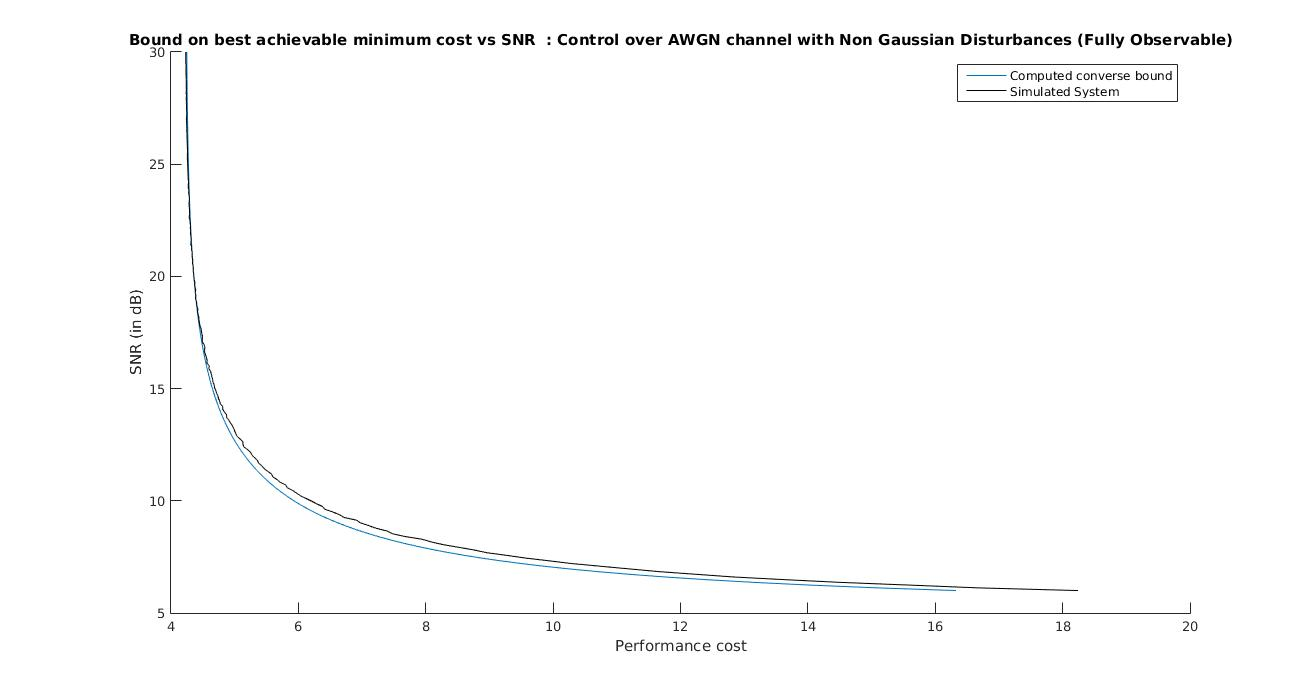
\includegraphics[scale=0.27]{laplaceW_bound_simulation_withoutV}
			  \caption{Comparing the computed optimal cost with the simulated optimal cost for system with AWGN communication channel. The fully observable system has the parameter $A = 2$ and the system disturbance $w$ is zero mean Laplacian with $\sigma_{w} = 1$.}
			 \label{lowerbound_vs_laplace}
		\end{figure}	
		We also studied the partially observable case where (i.e. $y = x + v$) in a similar fashion. The results for partially observable system and for different system parameters and distributions of $w$ are available at the web link given in \cite{git}.
%		 Similarly, for the partially observable case (i.e. $y = x + v$), we have the modified lower bound from \cite{victoria} given in Eq.(\ref{lowerbound_v})
%			  \begin{align}
%			  \label{lowerbound_v}
%			  \mathbb{R}(b) &\geq \log(|det(A)|) + \frac{n}{2} \log \left( 1 + \frac{\left(|det(C(T-\Sigma_{W})C^{T} + \Sigma_{V})|^{\frac{1}{n}} + |detC^{T}C|^{\frac{1}{n}}N(w)\right)|det KM|^{\frac{1}{n}}}{(b-b_{min})/n}\right)\\
%			  \intertext{For the scalar case with $n = 1$ and $C = 1$, we have}
%			  \mathbb{R}(b) &\geq \log|A| + \frac{1}{2} \log \left( 1 + \frac{\left(|(T-\Sigma_{W}) + \Sigma_{V}| + N(w)\right)KM}{b-b_{min}}\right)
%			  \end{align}
%			  where $T,\Sigma_{V}, \Sigma_{W}, K, M$ are obtained by solving AREs for classical LQG control. For details see \cite{victoria}.\\
%			  Using the channel capacity concept as for the fully observable case, we convert the lower bound in Eq.(\ref{lowerbound_v}) to get an expression for cost with the SNR of the AWGN channel for the partially observable case. 
% The plot comparing the simulation and computed lower bound for partially observable case is given in Fig.(\ref{lowerbound_vs_laplace_v})
%			  \begin{figure}[H]
%			  \centering
%			 \tiny{	
%%			  \resizebox{5in}{!}{\input{lowerBound_Simulation_rateLimitedLQG.pdf_tex}}
%			\includesvg[width=16cm]{laplaceW_bound_simulation_withV}}
%%			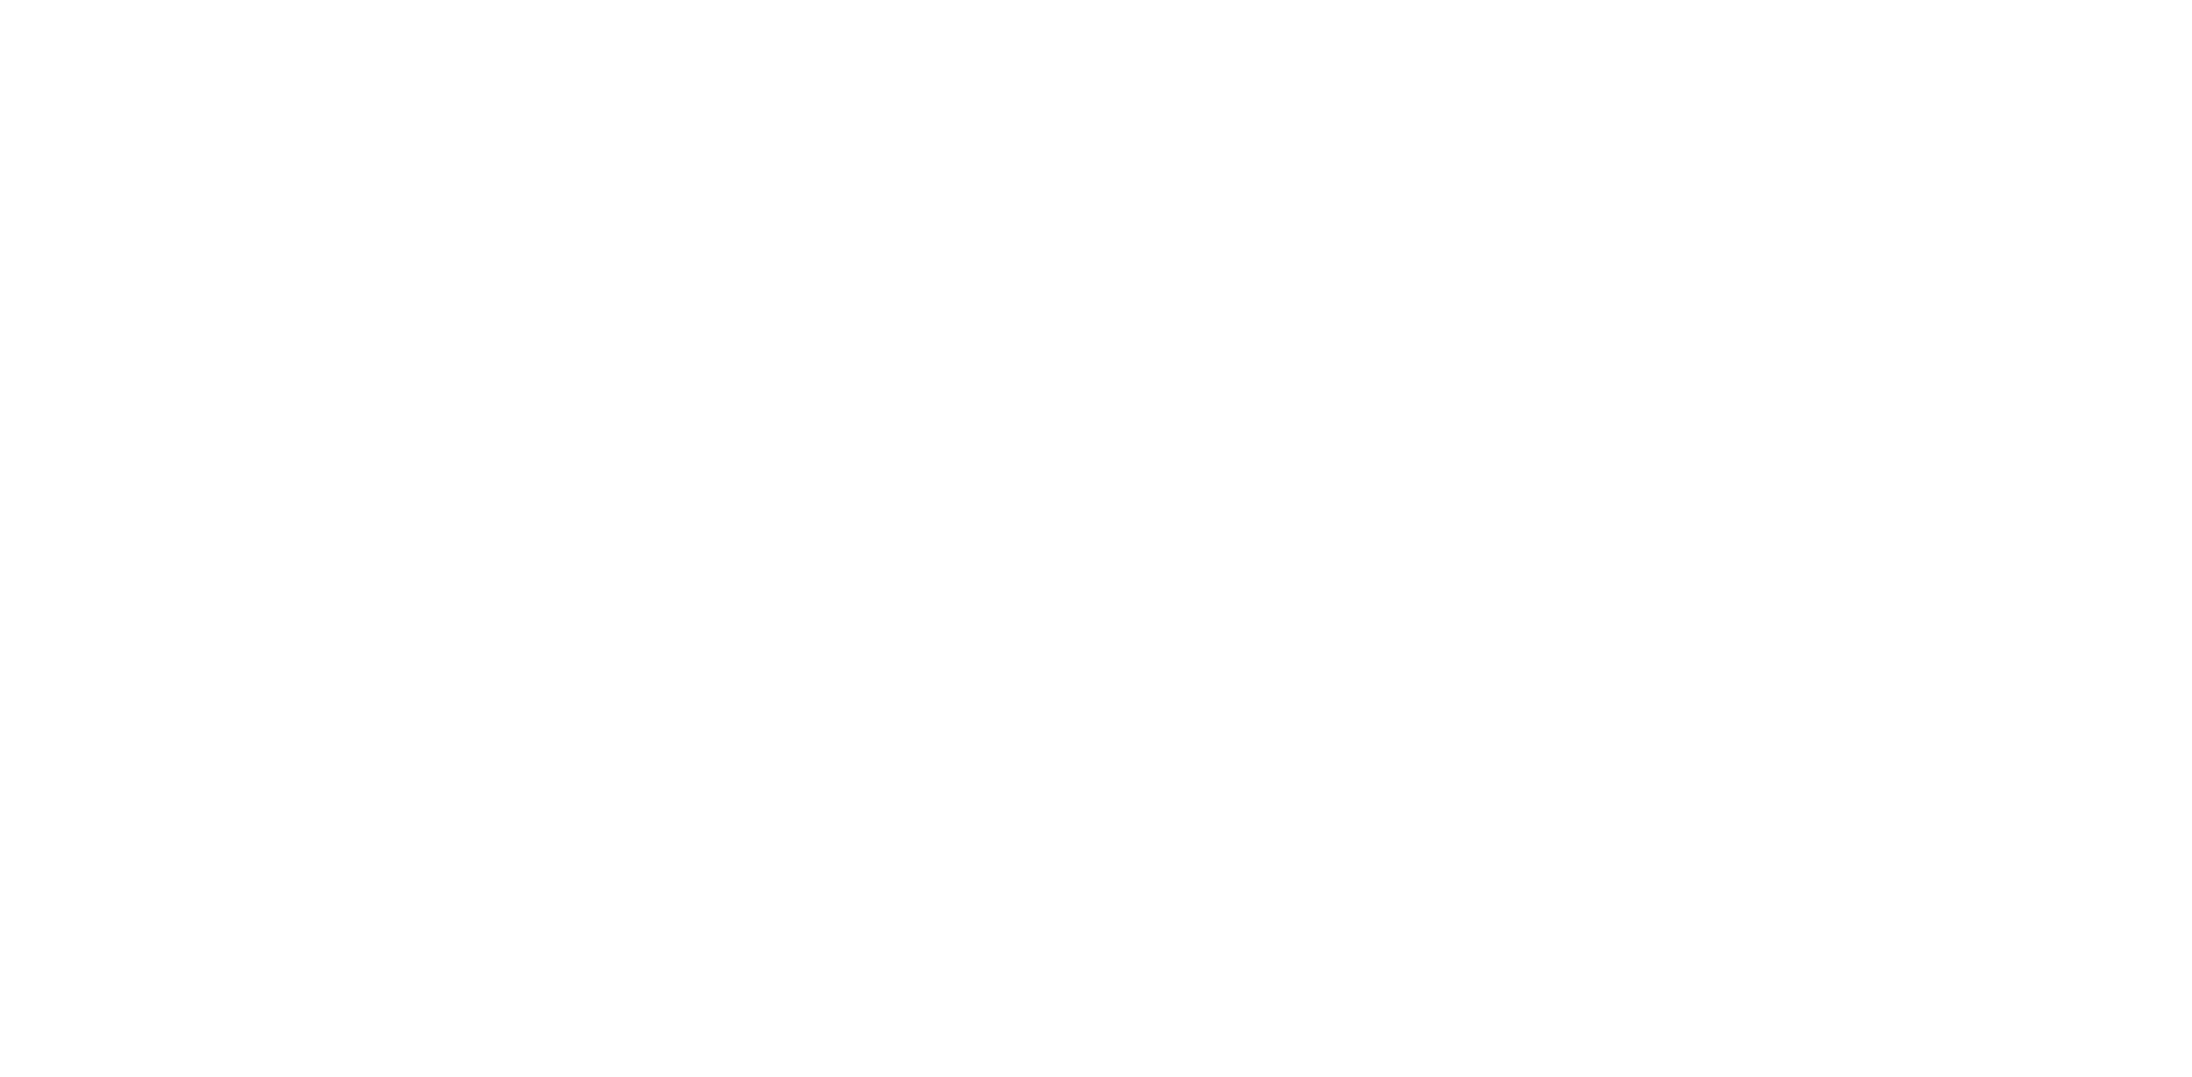
\includegraphics[scale=0.27]{laplaceW_bound_simulation_withV}
%			  \caption{Comparing the computed optimal cost with the simulated optimal cost for system with AWGN communication channel. The partially observable system has the parameter $A = 2$, the system disturbance $w$ is zero mean Laplacian with $\sigma_{w} = 1$ and observation noise is assumed to be zero mean Gaussian with $\sigma_{v} = 1$}
%			 \label{lowerbound_vs_laplace_v}
%		\end{figure}	
		
\chapter{Rate-Limited Communication Channel Constraint}

		Similar to the AWGN channel case, our approach to studying the tradeoff in the rate-limited channel case involves using the lower bound from \cite{victoria}, Eq.(\ref{lowerbound}) and Shannon's channel capacity concept. We demonstrated the tightness of the bound by using a simple uniform quantization scheme to implement the rate-limited communication. We observed that the lower bound is closely followed with this scheme. Towards the end of this section, we also present some initial results on a similar tradeoff study for a system with uncertain parameter $A$, which has a known probability distribution in the same setting of rate-limited communication between the observer and the controller. 
		\\We approximated the rate-distortion function ($R(b)$ in the bound, See Eq.(\ref{lowerbound}) using the quantizer entropy. To calculate the output entropy of the quantizer in the simulated system, we estimated the probabilities of each sample falling in the different quantization bins. Using the expression of entropy $H(x) = \sum\limits_{i} P_{i}(x)\log\left(\frac{1}{P_{i}(x)}\right)$, we calculated the entropy of the quantizer output for each $\Delta$, the quantizer step size. The simulated system was then compared with the bound, the result is shown in the Fig.(\ref{lowerboundQ_sim}).
		\begin{figure}[H]
			  \centering
%			  \includesvg[width=1.0\textwidth]{block2}
%			  \def\svgscale{5.5}
%			  \tiny{
			  \resizebox{15cm}{!}{\input{lowerBound_Simulation_rateLimitedLQG.pdf_tex}}
%			\includesvg[width=14cm]{lowerBound_Simulation_rateLimitedLQG}}
			  \caption{Comparing the lower bound to the computed optimal cost with the simulated optimal cost for system with rate-limited channel. The fully observable system has the parameter $A = 2$, and the system disturbance $w$ is zero mean Gaussian with $\sigma_{w} = 1$}
			 \label{lowerboundQ_sim}
		\end{figure}	
		The result for partially observable case is shown in Fig.(\ref{lowerboundQ_sim_v}).
		\begin{figure}[H]
			  \centering
%			  \includesvg[width=1.0\textwidth]{block2}
%			  \def\svgscale{5.5}
%			  \tiny{
			 \resizebox{15cm}{!}{\input{lowerBound_Simulation_GaussianDist_rateLimited_partiallyObservedLQG.pdf_tex}}
%			\includesvg[width=14cm]{lowerBound_Simulation_GaussianDist_rateLimited_partiallyObservedLQG}}
			  \caption{Comparing the lower bound to the computed optimal cost with the simulated optimal cost for system with rate-limited channel. The partially observable system has the parameter $A = 2$, the system disturbance $w$ is zero mean Gaussian with $\sigma_{w} = 1$ and observation noise is assumed to be zero mean Gaussian with $\sigma_{v} = 1$}
			 \label{lowerboundQ_sim_v}
		\end{figure}	
Further results showing the upper bound as well along with lower bound and simulated system are available on the web link \cite{git}. Other results also include simulations for different system parameters and different probablity distributions for the system disturbance $w$. 
%	To study the tightness of the upper bound, first we show the plot comparing the lower bound and the upper bound in Fig.(\ref{lower_upper}).
%	\begin{figure}[H]
%
%			  \centering
%%			  \includesvg[width=1.0\textwidth]{block2}
%%			  \def\svgscale{5.5}
%			  \tiny{
%%			  \input{ulft.pdf_tex}}
%			\includesvg[width=16cm]{lowerBound_upperBound}}
%%			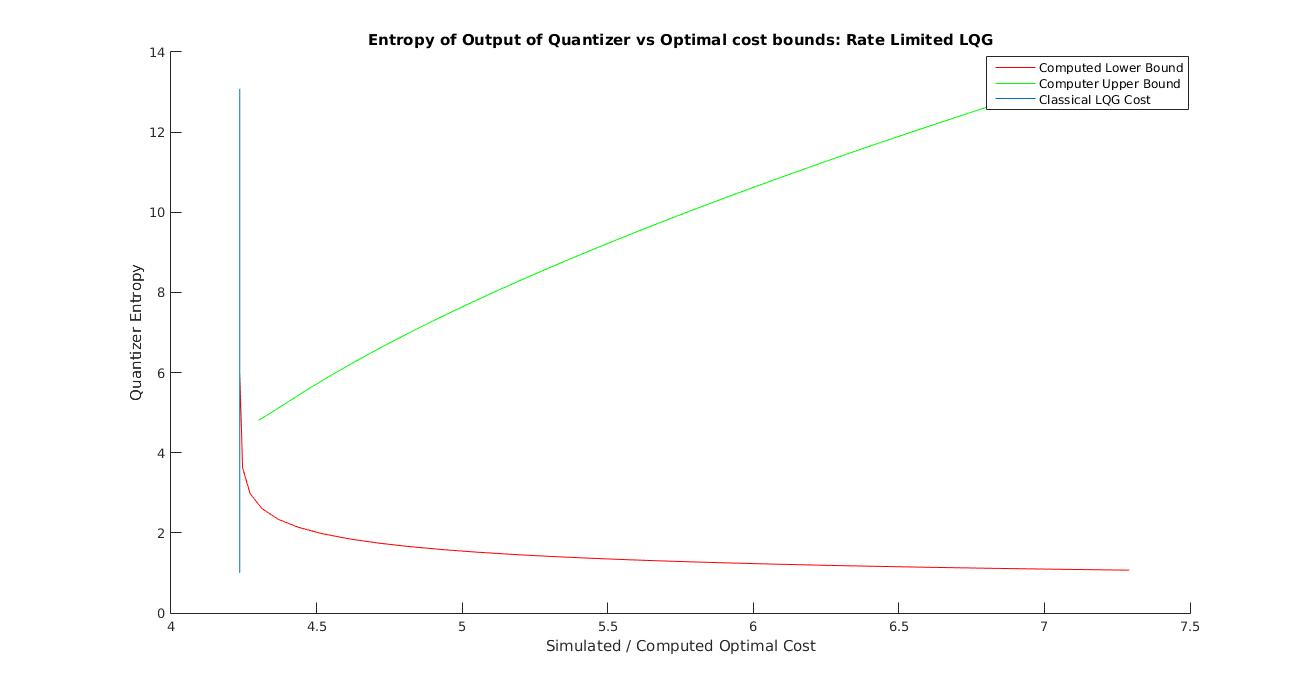
\includegraphics[scale=0.33]{lowerBound_upperBound}
%			  \caption{Comparing the lower bound and upper bound to the optimal cost in the rate limited channel case. The fully observable system has the parameter $A = 2$ and the system disturbance $w$ is zero mean Gaussian with $\sigma_{w} = 1$}
%			 \label{lower_upper}
%		\end{figure}	
%		To study the tightness of the bounds, we plot the lower bound, the upper bound and the curve for simulation of the system with a uniform quanitzer, as shown in Fig.(\ref{lower_upper_sim}).
%		\begin{figure}[H]
%			  \centering
%%			  \includesvg[width=1.0\textwidth]{block2}
%%			  \def\svgscale{5.5}
%			  \tiny{
%%			  \input{ulft.pdf_tex}}
%			\includesvg[width=16cm]{lowerBound_Simulation_UpperBound}}
%			  \caption{Comparing the lower bound and upper bound to the optimal cost in the rate limited channel case with the system simulation for simple uniform quantization scheme. The fully observable system has the parameter $A = 2$ and the system disturbance $w$ is zero mean Gaussian with $\sigma_{w} = 1$}
%			 \label{lower_upper_sim}
%		\end{figure}	
%		
%		The plots shown above are not restricted to a particular distribution of $w$, to demonstrate the fact, the following figures have been given for the case where system disturbance has a Laplace distribution. 
%		\begin{figure}[H]
%
%			  \centering
%%			  \includesvg[width=1.0\textwidth]{block2}
%%			  \def\svgscale{5.5}
%			  \tiny{
%%			  \input{ulft.pdf_tex}}
%			\includesvg[width=16cm]{lowerBound_upperBoundL}}
%%			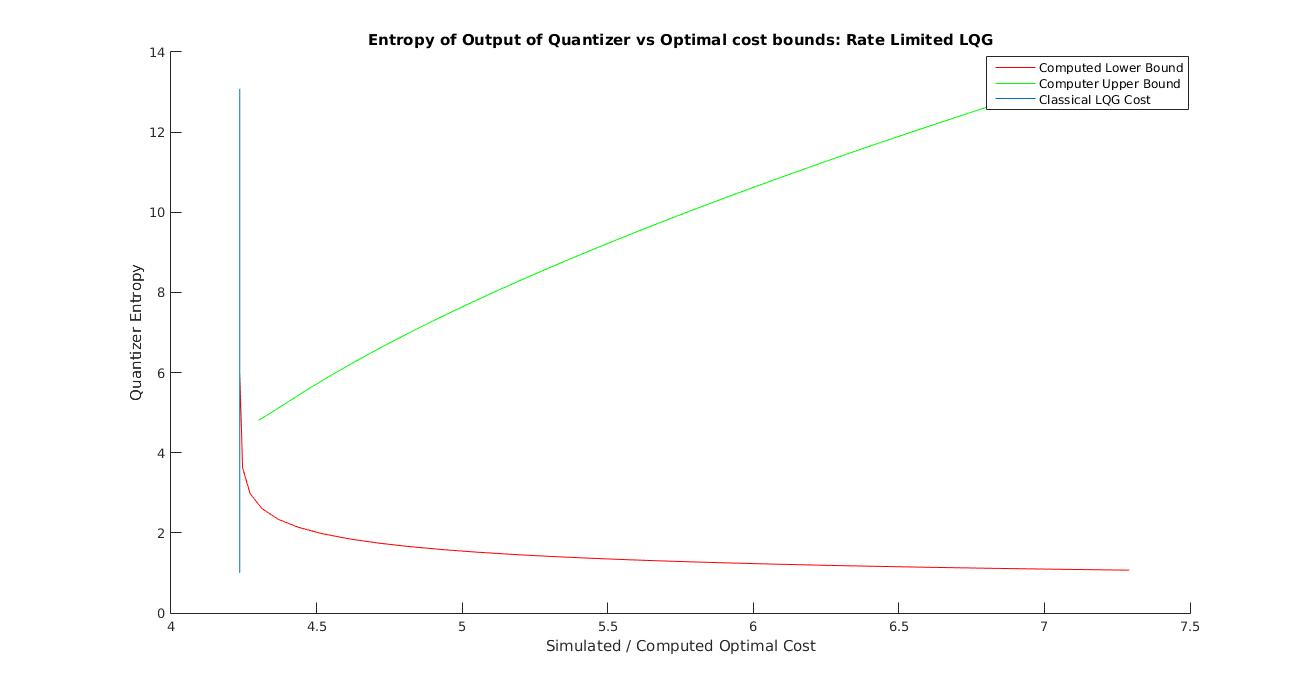
\includegraphics[scale=0.33]{lowerBound_upperBound}
%			  \caption{Comparing the lower bound and upper bound to the optimal cost in the rate limited channel case. The fully observable system has the parameter $A = 2$ and the system disturbance $w$ is zero mean Laplacian with $\sigma_{w} = 1$}
%			 \label{lower_upper}
%		\end{figure}	
%		\begin{figure}[H]
%			  \centering
%%			  \includesvg[width=1.0\textwidth]{block2}
%%			  \def\svgscale{5.5}
%			  \tiny{
%%			  \input{ulft.pdf_tex}}
%			\includesvg[width=16cm]{lowerBound_Simulation_Laplace_Disturbance}}
%			  \caption{Comparing the lower bound to the computed optimal cost with the simulated optimal cost for system with rate limited channel. The fully observable system has the parameter $A = 2$, and the system disturbance $w$ is zero mean Laplacian with $\sigma_{w} = 1$}
%			 \label{lowerboundQL_sim}
%		\end{figure}	
%		\begin{figure}[H]
%			  \centering
%%			  \includesvg[width=1.0\textwidth]{block2}
%%			  \def\svgscale{5.5}
%			  \tiny{
%%			  \input{ulft.pdf_tex}}
%			\includesvg[width=16cm]{lowerBound_Simulation_LaplaceDist_rateLimited_partiallyObservedLQG}}
%			  \caption{Comparing the lower bound to the computed optimal cost with the simulated optimal cost for system with rate limited channel. The partially observable system has the parameter $A = 2$, the system disturbance $w$ is zero mean Laplacian with $\sigma_{w} = 1$ and observation noise is assumed to be zero mean Gaussian with $\sigma_{v} = 1$}
%			 \label{lowerboundQL_sim_v}
%		\end{figure}	
%	\begin{figure}[H]
%
%			  \centering
%%			  \includesvg[width=1.0\textwidth]{block2}
%%			  \def\svgscale{5.5}
%%			  \tiny{
%%			  \input{ulft.pdf_tex}}
%			\includegraphics[scale=0.5]{}
%			  \caption{Comparing the lower bound and upper bound to the optimal cost in the rate limited channel case. The fully observable system has the parameter $A = 2$ and the system disturbance $w$ is zero mean Laplacian with $\sigma_{w} = 1$}
%			 \label{lower_upperL}
%		\end{figure}	
%		\begin{figure}[H]
%			  \centering
%%			  \includesvg[width=1.0\textwidth]{block2}
%%			  \def\svgscale{5.5}
%			  \tiny{
%%			  \input{ulft.pdf_tex}}
%			\includesvg[width=16cm]{loweruppersimlaplace}}
%			  \caption{Comparing the lower bound and upper bound to the optimal cost in the rate limited channel case with the system simulation for simple uniform quantization scheme. The fully observable system has the parameter $A = 2$ and the system disturbance $w$ is zero mean Laplacian with $\sigma_{w} = 1$}
%			 \label{lower_upper_simL}
%		\end{figure}	
		
\section{Multiplicative Parameter Uncertainty in the Plant}
	The system parameter $A$ might itself be uncertain having a known probability distribution. This is often the case in digital control systems which inherently have white parameters occuring due to sampling period or in some controller parameters. There are various known examples of economic systems as well which exhibit uncertain system parameters. The issue of stabilizability of such systems has been a topic of research since the 1970s (see \cite{utp}). Because of the wide applications of these kind of systems, there have been many studies focused on general LQG control design for such systems. However the most general case where the system is partially observable and the system parameter $A$ has a probability distribution has been an unsolved problem. As described in \cite{berstekas} and other related research papers, the separation theorem which plays a major role in LQG control design is not valid for the system with uncertain parameter. Although the partially observable case with random system parameter(s) remains unsolved, the effect of communication between the observer and the controller has been a focus of recent research in this area. In \cite{victoria2}, stabilizability conditions have been derived for such a system and a rate-distortion bound similar to Eq.(\ref{lowerbound}) has been given. To study the tradeoff between the rate of communication and the optimal achievable LQG cost, we compared the uniform quantizer entropy with the bound (similar to the rate-limited case). The result is shown in Fig.(\ref{bound_randomA}). 
	\begin{figure}[H]
			  \centering
%			  \includesvg[width=1.0\textwidth]{block2}
%			  \def\svgscale{5.5}
%			  \tiny{
			  \resizebox{15cm}{!}{\input{multiplicative_randomness_rate_limited.pdf_tex}}
%			\includesvg[width=14cm]{multiplicative_randomness_rate_limited}}
			  \caption{Comparing the lower bound to the optimal cost in the rate-limited channel case with uncertain system parameter $A$ using a uniform quantization scheme. The fully observable system has the parameter $A = 2$ and the system disturbance $w$ is zero mean Gaussian with $\sigma_{w} = 1$}
			 \label{bound_randomA}
		\end{figure}	
		
	As we can see that the uniform quantizer in this case does not follow the bound as closely as we observed when $A$ was fixed. In order to improve the performance we improved the quantizer design by using the Lloyd-Max quantizer for a fixed number of points. Some results with this quantizer are available in \cite{git}.
\chapter{Conclusions and Future Work}
\section{For AWGN channel}
As expected, for high SNR values, the optimal cost achieved was lower. This was exhibited in all of the results as the cost tends to the minimum value in the high SNR regime.  The important inference that can be drawn from the comparison between the simulations and the lower bound given in \cite{victoria} is that the lower bound is tight for non Gaussian system disturbance $w$ as well. We demonstrated this result for both partially observable and fully observable cases. Hence, we can say that the lower bound given in \cite{victoria} is tight for non-Gaussian $w$'s as well. \\
We only considered a scalar system with only a single channel of communication between the observer and the controller. It would be interesting to study the tradeoff for MIMO (multi-input and multi-output) systems as well as when there are more than one channels available to transmit the information. The optimal power allocation over multiple channels would be an interesting problem to solve. 

\section{Rate-Limited Channel}
Similar to the AWGN case, it was expected that for higher entropy of the output of the quantizer (i.e. smaller quantization bins), the optimal cost would tend to the minimum. The results obtained are in line with this expectation, as we observed that the optimal cost tends to the minimum cost ($b_{min}$) for higher values of quantizer entropy. The major conclusion is that even on using the simplest of schemes for quantization (a uniform quantizer), we observed that the performance cost values were quite close to the lower bounds given in \cite{victoria} both for partially observable and fully observable case. \\


%\begin{figure}[hbt!]
%\centering
%
\includegraphics[width=.3\textwidth]{caltech.png}
%\caption{This is a figure}\label{fig:logo}
%\index{figures}
%\end{figure}


%\begin{table}[hbt!]
%\centering
%\begin{tabular}{ll}
%\hline
%Area & Count\\
%\hline
%North & 100\\
%South & 200\\
%East & 80\\
%West & 140\\
%\hline
%\end{tabular}
%\caption{This is a table}\label{tab:sample}
%\index{tables}
%\end{table}


%\endnote{Endnotes are notes that you can use to explain text in a document.}



\printbibliography[heading=bibintoc]
%
%\appendix

%\chapter{Questionnaire}
%\chapter{Consent Form}

%\printindex
%
%\theendnotes*
%
%%% Pocket materials at the VERY END of thesis
%\pocketmaterial
%\extrachapter{Pocket Material: Map of Case Study Solar Systems} 
%

\end{document}
